\subsection{Własności wykorzystywanych materiałów}
W układach omawianych w poniższym rozdziale wykorzystywane są złoto i arsenek galu, dlatego ich własności omówione zostaną bardziej szczegółowo. Wszystkie przewodniki, w tym złoto, ze względu na czasy relaksacji rzędu $10^{-14}$s charakteryzują się niemal bezdyspersyją przewodnością. W związku z tym równanie (\ref{eq:lorenz-drude}) możemy zapisać w prostszej postaci
\begin{equation}
	\varepsilon(f)=\varepsilon_{\infty}+i \frac{\sigma_0}{\varepsilon_0 f},
	\label{eq:eps-met-thz}
\end{equation}
gdzie przez $\sigma_0$ oznaczona została przewodność. Dla złota w warunkach normalnych $\sigma_0=45.2 \frac{S}{\mu m}$.   Ze względu na znacznie większą wartość bezwzględną części urojonej od rzeczywistej dla obszaru subterahretzowego powyższe równanie (\ref{eq:eps-met-thz}) możemy dalej uprościć do postaci
\begin{equation}
	\varepsilon(f) \approx i \frac{\sigma_0}{\varepsilon_0 f}.
	\label{eq:eps-met-thz-app}
\end{equation}

\begin{figure}[tb]
	\begin{subfigure}{.45\textwidth}
		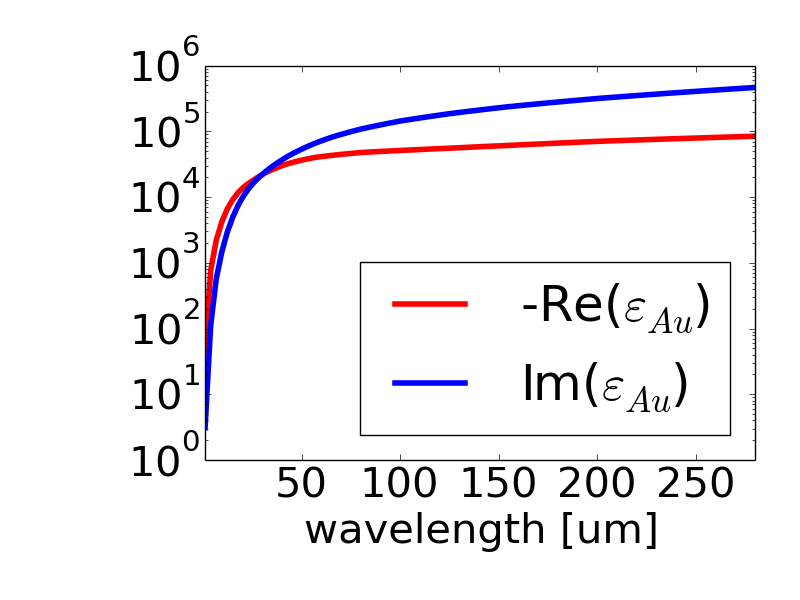
\includegraphics[width=\textwidth]{images/aueps.png}
		\caption{Zależność przenikalności elektrycznej od długości fali w zakresie od~$1$~do~$300$~THz, dla $Au$~\cite{ordal1983optical}}
		\label{fig:aueps}
	\end{subfigure}
	\begin{subfigure}{.45\textwidth}
		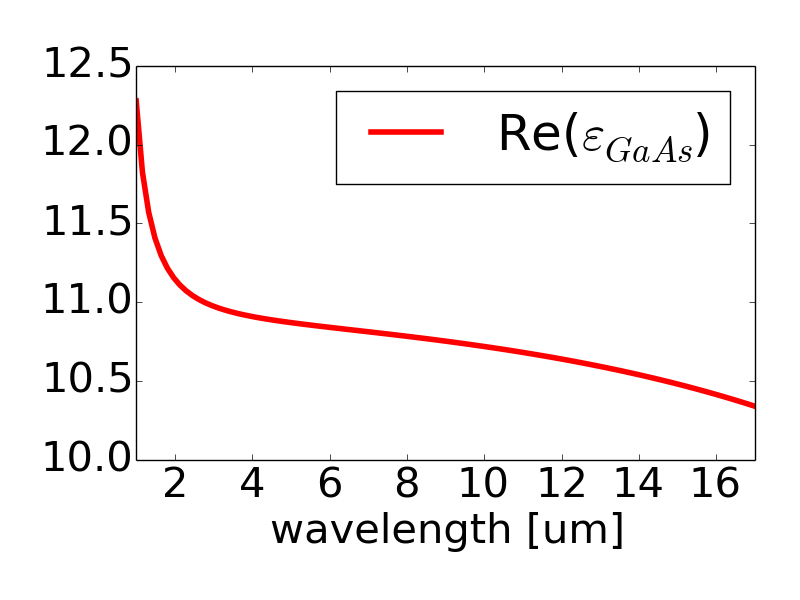
\includegraphics[width=\textwidth]{images/gaaseps.png}
		\caption{Zależność przenikalności elektrycznej od długości fali w zakresie, od~$17$~do~$300$~THz dla  $GaAs$~\cite{skauli2003improved}}
		\label{fig:gaaseps}
	\end{subfigure}
\end{figure}

Różnica w wartości bezwzględnej części rzeczywistej i urojonej przenikalności elektrycznej złota zmniejszają się ze wzrostem częstotliwości, dla $f=2THz$ moduł części rzeczywistej jest ok. 5 razy mniejszy od modułu części urojonej. Część rzeczywista przenikalności elektrycznej w omawianym zakresie jest ujemna a jej moduł zmienia się od $10^2$ do $10^4$. Ze względu na omówiony dominujący charakter części urojonej związanej z przewodnictwem eksperymentalne wyznaczenie przenikalności dielektrycznej jest bardzo trudne i nie zawiera częstotliwości poniżej $1$~THz~(długości fali powyżej $300$~$\mu$m)~\cite{ordal1983optical}\footnote{Powyższa analiza prawdziwa jest dla eksperymentów prowadzonych w temperaturze pokojowej, obniżenie temperatury do~$T=$80K powoduje wzrost przewodności złota do $\sigma_0=208\frac{S}{\mu m}$. W temperaturach kriogenicznych może w cienkich warstwach złota dominujący wpływ na przewodność może mieć rozpraszanie elektronów na defektach struktury.\cite{lide2009crc}}. Zależność $\varepsilon$ od długości fali została przedstawiona na wykresie \ref{fig:aueps}. Symulacje opisywane w poniższym rozdziale prowadzon są z maksymalną rozdzielczością $0.5$~$\mu$m na punkt obliczeniowy, natomiast głębokość naskórkowa dla $1$~THz $\delta=74.9$~nm~\cite{lee2009principles}. Mała głębokość naskórkowa w porównaniu do rozdzielczości uprawnia do przybliżenie złota przez doskonały przewodnik. 

W przeciwieństwie do złota warstwy $GaAs$ w zakresie THz mogą być traktowane jako bezstratne, charakteryzują się one również słabą dyspersją, a w przypadku obliczeń prowadzonych dla wąskiego zakresu długości fali może być traktowana jako stała. Warto jednak zwrócić uwagę, że warstwy $GaAs$ uzyskiwane w wyniku epitaksji z wiązki molekularnej poddawane są zazwyczaj procesowi wyżarzania~(ang.annealing) w celu ich wygładzenia lub eliminacji zanieczyszczeń. Proces ten może mieć jednak znaczący wpływ na koncentrację elektronów w paśmie przewodnictwa, co może znacząco zmienić właściwości elektromagnetyczne tego materiału~\cite{zhang2009annealing}. Zależność przenikalności elektrycznej $GaAs$ przedstawia wykres na rysunku \ref{fig:gaaseps}.


